\section{Analoger Aufbau}
Im Abschnitt (\ref{sec:d80}) wurde darauf hingewiesen, dass der Drumcomputer aus einem Sequenzer\footnote{ Schaltung die Folgen speichern und beliebig oft wiedergeben kann} und analogen Klangerzeugern besteht. Die Yamaha D80 verwendet im Wesentlichen zwei Schaltungen zur Umsetzung der Klangerzeugung. Im Folgenden werden diese technischen Umsetzungen genauer beschrieben, wobei das Bassdrum- und das Snaredrum-Modul im Fokus stehen, um die beiden Schaltungstypen zu erläutern.


Die vorhandene Schaltung aus der Yamaha Electron D80 modular zu nutzen, wurde sie an den Eurorack-Standard angepasst. Dies beinhaltete wie in der Einführung beschrieben die Änderung der Versorgungsspannung, des Triggers und der Ausgangsspannung. Des Weiteren wurde der Schaltplan um eine manuelle Ansteuerung durch einen Taster erweitert.

\subsection{Manueller Trigger}

Um eine bequeme und direkte Klangeinstellung zu ermöglichen, haben wir die Module mit einem manuellen Trigger erweitert. Hierfür wurde der NE555 Timerbaustein als monostabile Kippstufe und ein Taster genutzt, wie in der Abbildung (\ref{fig:Ne555}) dargestellt.


\begin{figure}[h]
    \centering
    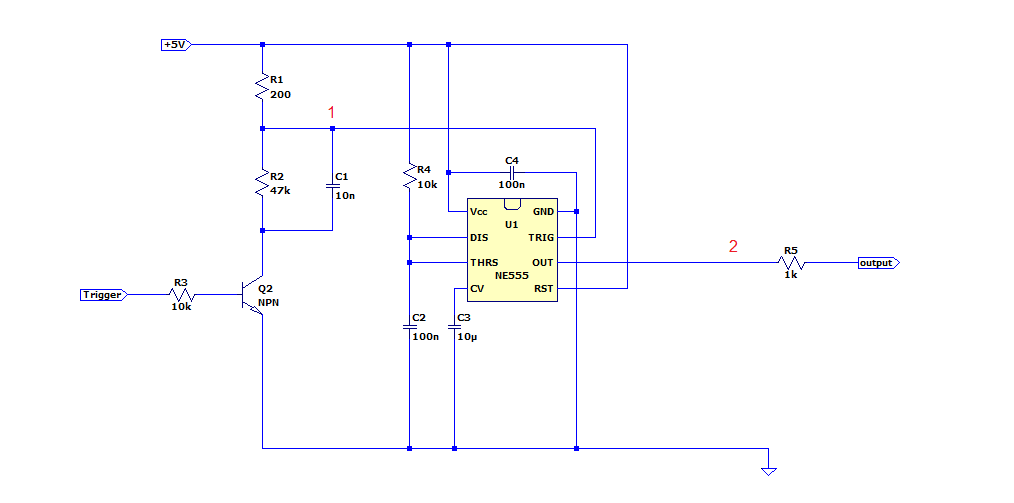
\includegraphics[width=1\textwidth]{Images/Ne555.png}
    \caption[Ne555]{NE555 Trigger Schaltung}
    \label{fig:Ne555}
\end{figure}

Da die Implementierung eines Tasters in LT Spice nicht möglich ist, wird die Funktionsweise mithilfe des Transistors Q2 erläutert.

Die Schaltung zur Klangerzeugung benötigt einen Triggerimpuls von etwa $1\,\unit{.\milli\second}$ Länge. Um diese Impulsdauer mit dem NE555 Timerbaustein zu erzeugen, muss der Triggereingang des NE555 eine kürzere Impulsdauer als am Ausgang haben. Hierfür wird die Parallelschaltung von R2 und C1 verwendet. Wenn der Transistor leitend wird, aufgrund eines beliebig langen Triggerimpulses, entlädt sich der Kondensator schnell. Durch die Wahl einer sehr kleinen Kapazität wird die Zeitkonstante entsprechend klein, und der Kondensator lädt sich schnell auf die Spannung über R2 wieder auf. Dies erfüllt die Bedingung einer kürzeren Impulsdauer am Eingang.
Die Ausgangsimpulsdauer des NE555 folgt weiterhin der Formel (\ref{eq:Impulsdauer}).

\begin{equation}
   \text{Impulsdauer:}\quad t_w=1.1 \cdot R_4 \cdot C_2
    \label{eq:Impulsdauer}
\end{equation}

Mit den vorliegenden Bauteilwerten erzeugt die Schaltung einen Impuls von $1,1\,\unit{\milli\second}$ Länge, wie im folgenden Simulationsausschnitt des Spannungsverlaufs nachvollzogen werden kann. Dabei repräsentiert der untere Verlauf die Spannung an Punkt 1 und der obere Verlauf die Spannung an Punkt 2 des Schaltplans in Abbildung (\ref{fig:Ne555}).

\begin{figure}[H]
    \centering
    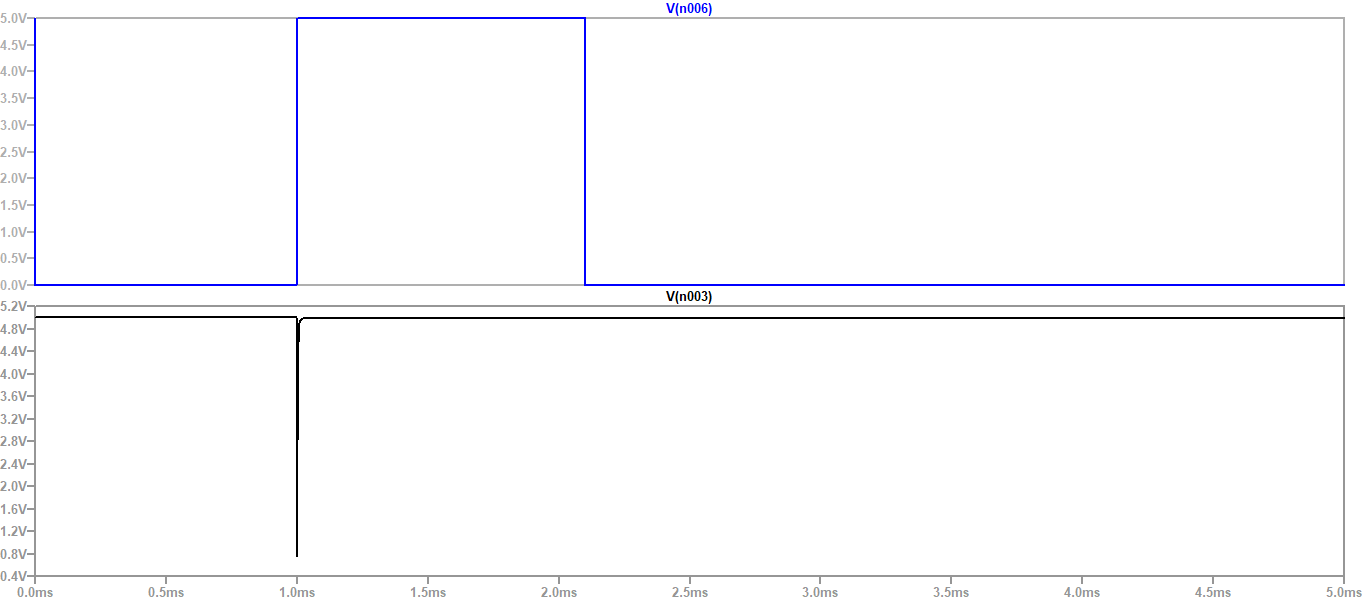
\includegraphics[width=0.8\textwidth]{Images/NE555_Spannungen.png}
    \caption[NE555 Spannungswerte]{NE555 Spannungswerte}
    \label{fig:Ne555_Spannung}
\end{figure}

\subsection{Klangerzeugung}

Mit diesem beschriebenen Impuls wird nun die eigentliche Schaltung zur Klangerzeugung ausgelöst. Im Folgenden wird unter Verwendung des Bassdrum-Moduls das allgemeine Prinzip der Klangerzeugung vorgestellt.

\begin{figure}[h]
    \centering
    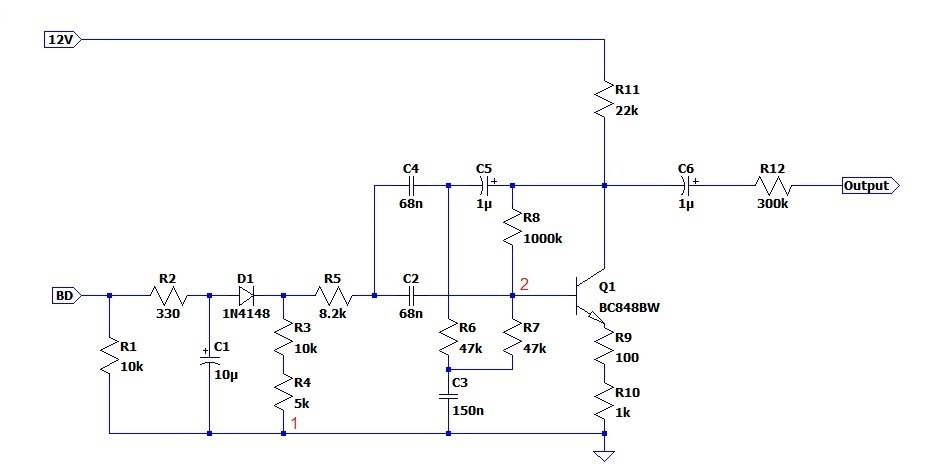
\includegraphics[width=1\textwidth]{Images/ltspice_bassdrum.jpg}
    \caption[Bassdrum Schaltplan]{Bassdrum Schaltplan}
    \label{fig:Bassdrum}
\end{figure}

Das Hauptprinzip dieser Schaltung basiert auf der Mitkopplung eines Notchfilters\footnote{besonders schmalbandiger Bandpassfilter} in der Transistorstufe. Bei genauerem Hinsehen erkennt man, dass das Notchfilter durch ein Doppel-T-Filter realisiert wurde. Ein Hinweis darauf ist, dass die Kondensatoren C2 und C4 etwa die halbe Kapazität von C6 haben und die Reihenschaltung aus R3, R4 und R5 den halben Widerstandswert von R6 und R7 besitzt. Dies trifft auch auf das Doppel-T-Filter zu, wie es in der folgenden Abbildung zu sehen ist.
\begin{figure}[H]
    \centering
    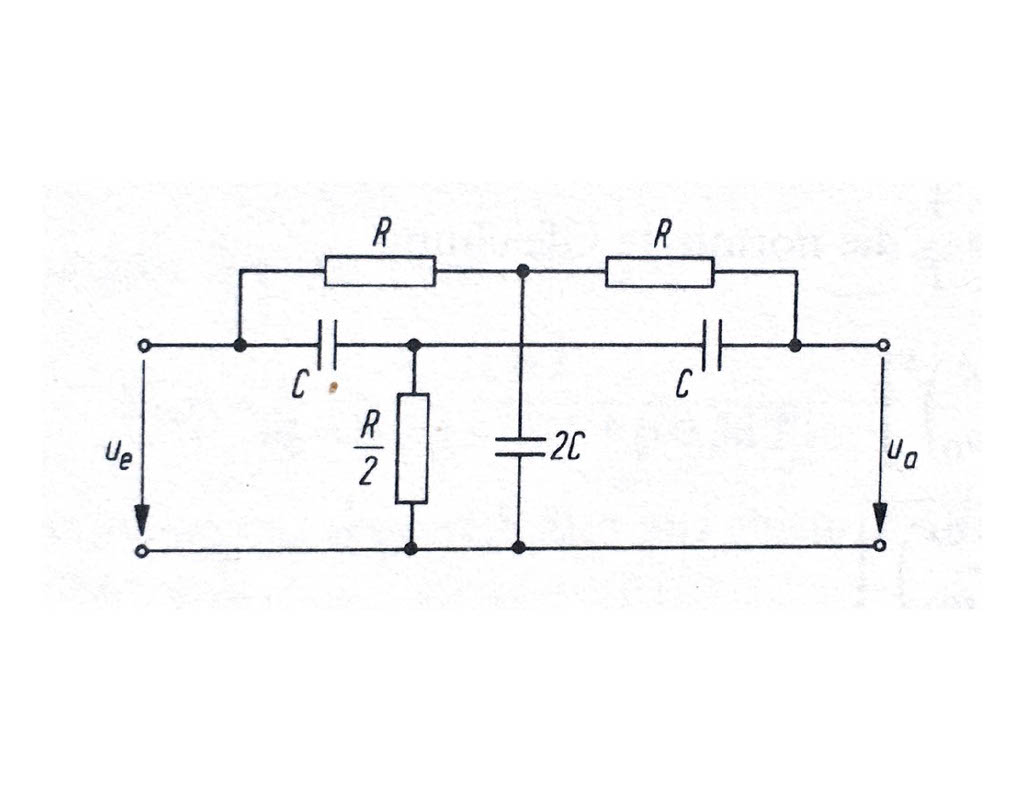
\includegraphics[width=0.8\textwidth]{Images/doppel T filter.jpg}
    \caption[Doppel T filter]{Doppel T filter \cite[s.41]{Bystron}}
    \label{fig:doppel T filter}
\end{figure}

Es lässt sich mithilfe der Formel (\ref{eq:Doppel T Filter Resonanzfrequenz}) die Resonanzfrequenz und somit die Tonhöhe der Bassdrum ermitteln. Mit den Bauteilwerten aus der Schaltung ergibt sich eine Resonanzfrequenz von 52,01 Hz.

\begin{equation}
   \text{Resonanzfrequenz} : v_o=\frac{1}{2*\pi*R*C}
    \label{eq:Doppel T Filter Resonanzfrequenz}
\end{equation}

Das Doppel-T-Filter besitzt des Weiteren eine ideale Phasenverschiebung von 180 Grad, wie im nachfolgenden Frequenzgang zu erkennen ist.
\begin{figure}[H]
    \centering
    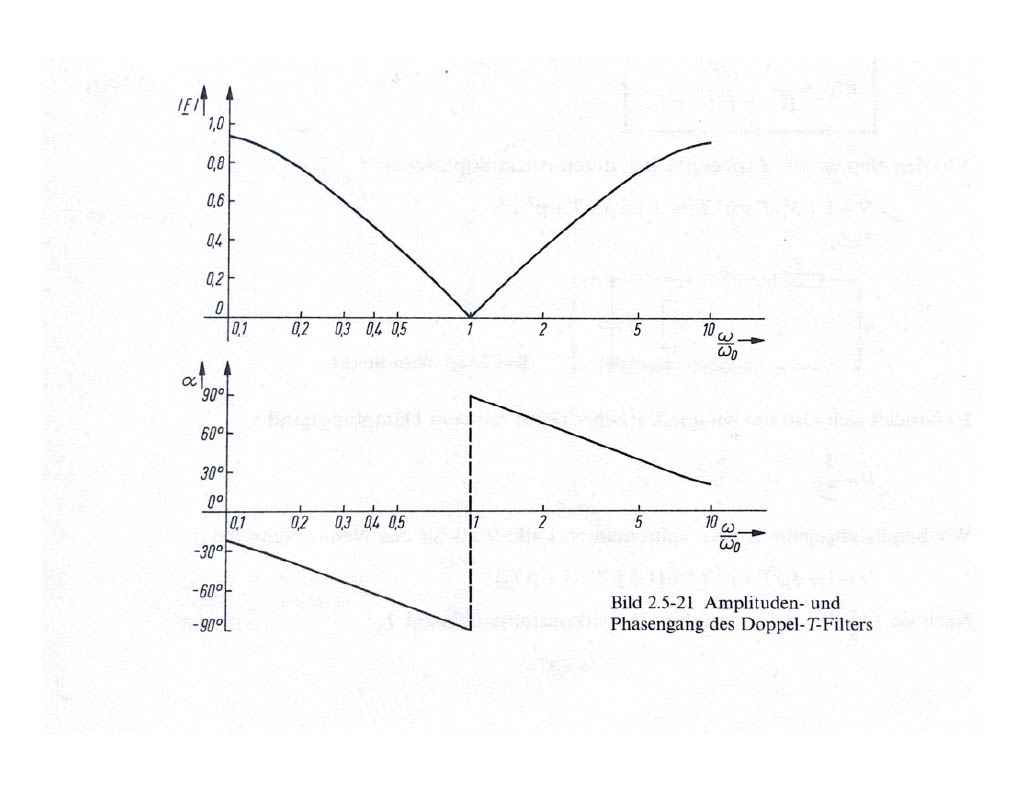
\includegraphics[width=1\textwidth]{Images/frequenzgang doppel t.jpg}
    \caption[Freuqunzgang Doppel T Filter]{Freuqunzgang Doppel T Filter \cite[s.41]{Bystron}}
    \label{fig:Freuqunzgang Doppel T Filter}
\end{figure}

Im nachfolgenden Bild ist der Frequenzgang zwischen Punkt 1 und Punkt 2 aus Abbildung (\ref{fig:Bassdrum}) zu sehen. Es ist ersichtlich, dass der Phasen- und Amplitudengang mit dem in Abbildung (\ref{eq:Doppel T Filter Resonanzfrequenz}) gezeigten Frequenzgang übereinstimmt, wobei aufgrund der Mitkopplung eine Spiegelung auftritt, die anstelle einer Abschwächung eine Verstärkung der Resonanzfrequenz bewirkt.

\begin{figure}[H]
    \centering
    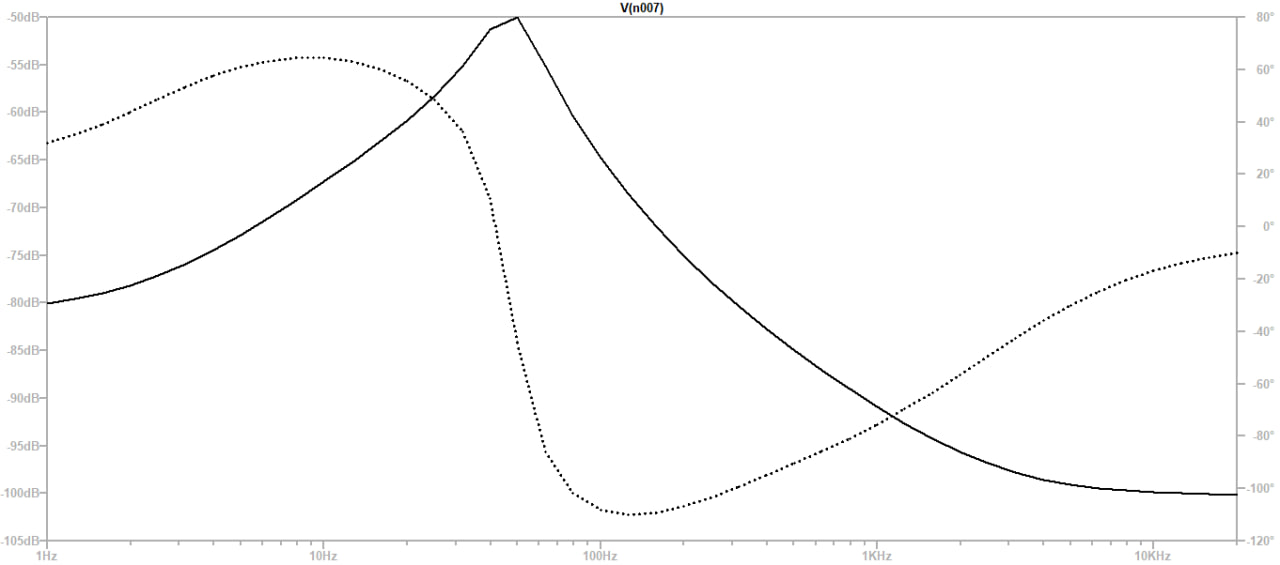
\includegraphics[width=0.8\textwidth]{Images/Frequenzgang Bassdrum.jpg}
    \caption[Frequenzgang Bassdrum]{Frequenzgang Bassdrum}
    \label{fig:Frequenzgang Bassdrum}
\end{figure}

Durch die Verschaltung des Transistors erfolgt zusätzlich eine Phasenverschiebung von 180 Grad. Idealerweise würde dies zu einer Gesamtphasenverschiebung von 360 Grad führen, was aufgrund der Mitkopplung in der Transistorstufe dazu führt, dass die Schaltung zu oszillieren beginnt. Durch die gezielte Auswahl der Widerstands- und Kondensatorwerte wird eine Phasenverschiebung erzeugt, die weniger als 360 Grad beträgt. Dies hat zur Folge, dass die Schwingung keine konstante Amplitude aufweist und im Laufe der Zeit abklingt. Die Widerstände R8 bis R11 dienen zur Einstellung des Arbeitspunkts und der Verstärkung, während mit dem Kondensator C5 das Signal wieder Eingekoppelt wird.

Im nachfolgenden Spannungs-Zeit-Verlauf kann nachvollzogen werden, wie die Schwingung aussieht, wobei der Spannungswert nach dem Entkopplungskondensator C6 in LT Spice dargestellt wurde. Hier wird auch deutlich, dass die Schwingung keine konstante Amplitude
aufweist und im Laufe der Zeit abklingt.

\begin{figure}[H]
    \centering
    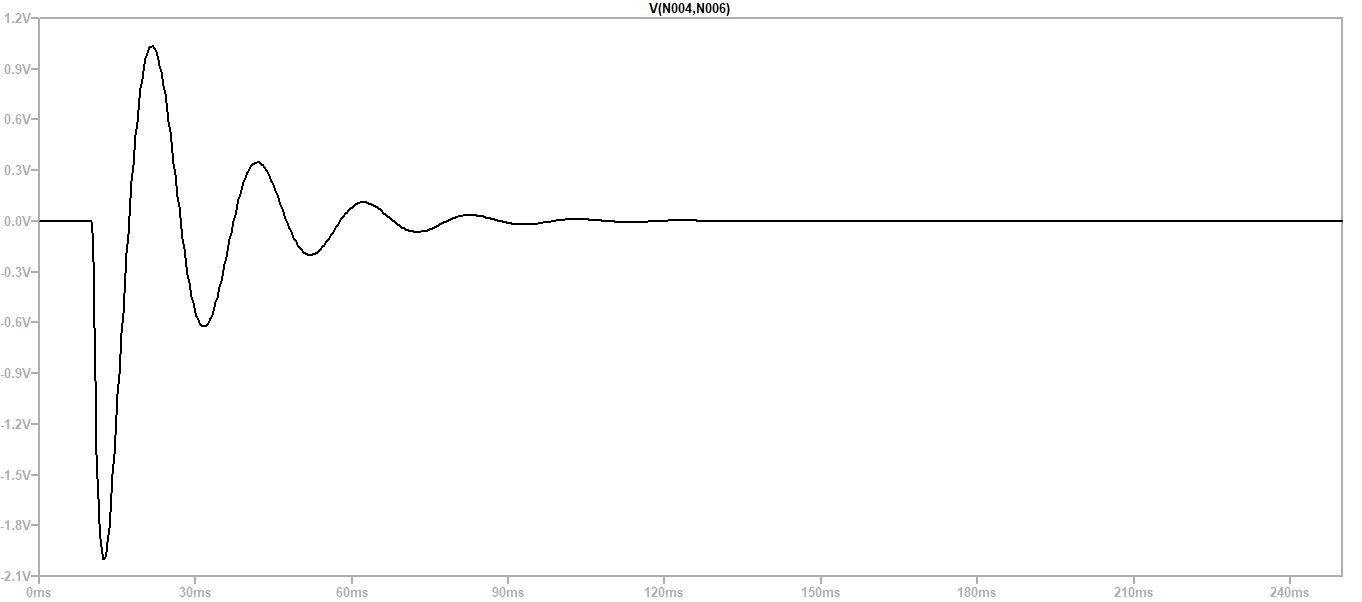
\includegraphics[width=0.8\textwidth]{Images/Bassdrum V t.png}
    \caption[Spannungsverlauf Bassdrum]{Spannungsverlauf Bassdrum}
    \label{fig:Spannungsverlauf Bassdrum}
\end{figure}


Nachdem die Bassdrum erläutert wurde, wird nun das Snaredrum-Modul behandelt. Das überarbeitete und angepasste Schaltungsschema ist im folgenden Bild dargestellt.

\begin{figure}[H]
    \centering
    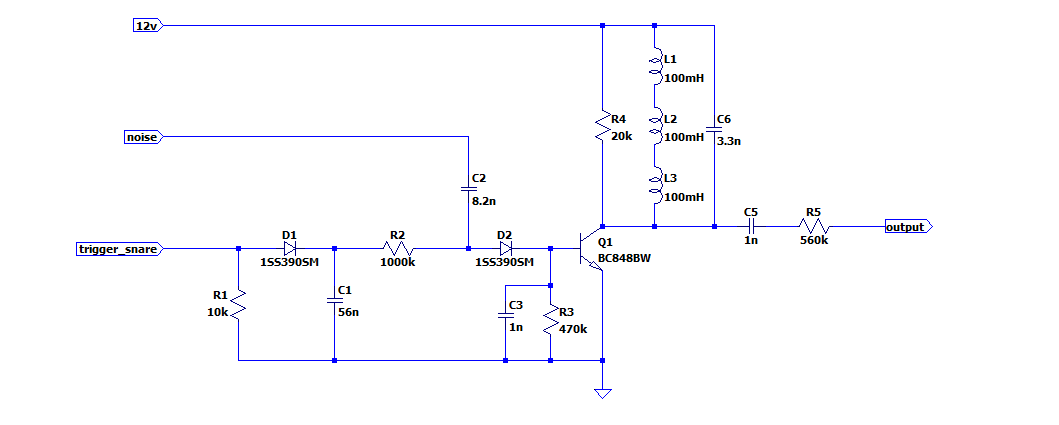
\includegraphics[width=1\textwidth]{Images/SD_Noise.png}
    \caption[Snaredrum Schaltplan]{Snaredrum Schaltplan\cite{ServiceManual}}
    \label{fig:SD_noise}
\end{figure}
Die Funktionsweise unterscheidet sich von der des Bassdrum-Moduls. Hier erfolgt eine Überlagerung des Triggerimpulses mit Rauschen, welches anschließend verstärkt und mithilfe eines Parallel-Schwingkreises zum Schwingen angeregt wird. Da LT Spice nicht in der Lage ist, die Rauschschaltung zu simulieren, wird der Rauschgenerator anhand des Originalschaltplans erläutert. Im nachfolgenden Bild ist der Schaltplan des Rauschgenerators aus der Yamaha D80 zu sehen.

\begin{figure}[H]
    \centering
    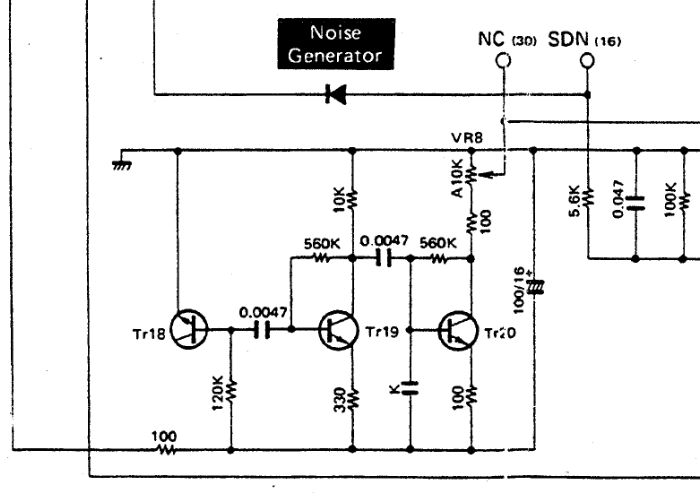
\includegraphics[width=0.6\textwidth]{Images/Noise Generator.png}
    \caption[Rauschgenerator]{Rauschgenerator\cite{ServiceManual}}
    \label{fig:Rauschgenerator}
\end{figure}

Das zentrale Element der Rauscherzeugung ist der Transistor Tr18. Bemerkenswert ist, dass aufgrund der Versorgungsspannung von -15 V das höhere Potenzial am Ground liegt und somit ein Stromfluss vom Ground zur Versorgungsspannung stattfindet. Es ist ersichtlich dass die Emitter-Basis-Strecke der Transistors genutzt wird, während der Kollektor-Pin unverbunden bleibt. Wenn die Durchbruchspannung der Emitter-Basis-Strecke von 5 V überschritten wird, erzeugt dies einen zufälligen Stromfluss an der Basis des Transistors. Durch den 120 k$\Omega$ Widerstand wird der zufällige Stromfluss zu einer Spannung welche als weißes Rauschen gemessen werden kann. Der Rest der Schaltung dient der Verstärkung und Filterung des Rauschsignals.

Im folgenden Abschnitt wird die Ausgangsspannung des Snaredrum-Moduls dargestellt. Es ist deutlich erkennbar, dass der Parallel-Schwingkreis nach dem Transistor Q1 den mit Rauschen überlagerten Triggerimpuls zum Schwingen anregt und nach kurzer Zeit aufgrund der Dämpfung durch R4 zum Ausklingen bringt. Mit Hilfe der Thomsonschen Schwingungsgleichung (\ref{eq:Thomsonsche Schwingungsgleichung}) für die Resonanzfrequenz lässt sich die Stimmung der Snaredrum bestimmen. Diese Beträgt 5058 Hz was typisch für eine Snare ist.

\begin{equation}
   \text{Thomsonsche Schwingungsgleichung:} f_o=\frac{1}{2*\pi\sqrt{L*C}}
    \label{eq:Thomsonsche Schwingungsgleichung}
\end{equation}


\begin{figure}[H]
    \centering
    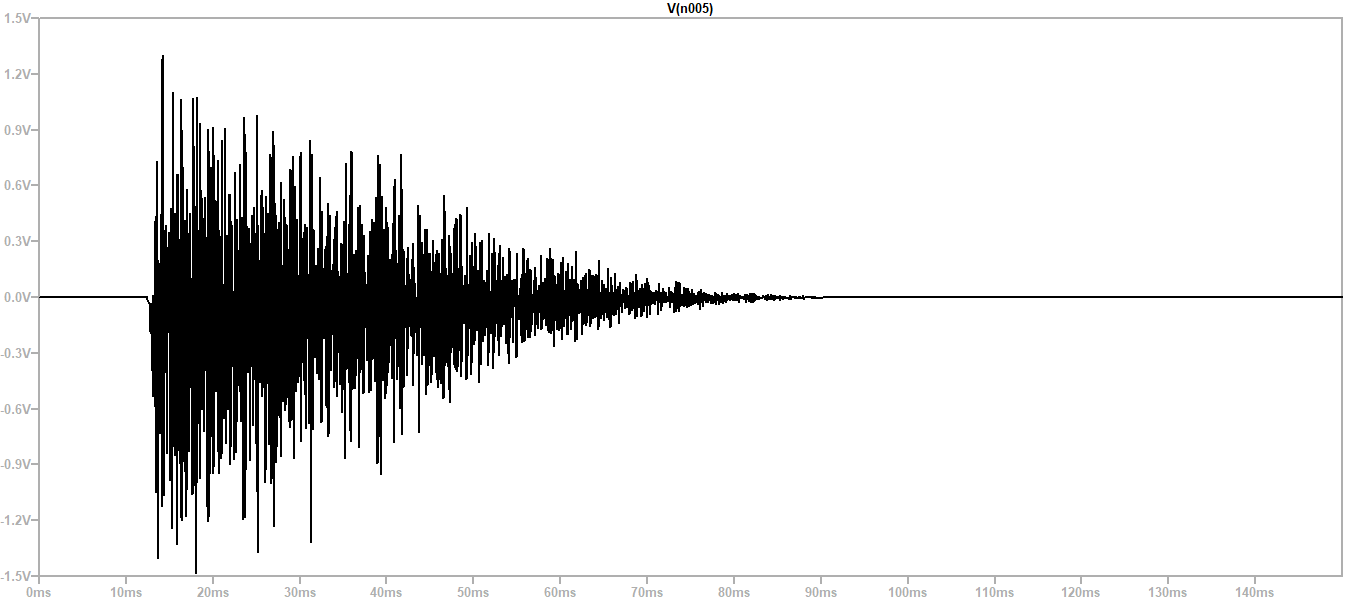
\includegraphics[width=0.8\textwidth]{Images/SD_N_Spice.png}
    \caption[Spannungsverlauf Snaredrum]{Spannungsverlauf Snaredrum}
    \label{fig:Spannungsverlauf Snaredrum}
\end{figure}


Wie in Abbildung (\ref{fig:Spannungsverlauf Bassdrum}) und Abbildung (\ref{fig:Spannungsverlauf Snaredrum}) zu sehen ist, beträgt die Ausgangsspannung etwa $5\,\unit{V_{pp}}$. Um den Eurorack-Standard von $10\,\unit{V_{pp}}$ zu erreichen, wurde eine nicht-invertierende Operationsverstärkerschaltung am Ausgang jeder Schaltung hinzugefügt.